% Sinh bởi report/scripts/bang_chuong4.py — không sửa tay.
\begin{figure}[H]
  \centering
  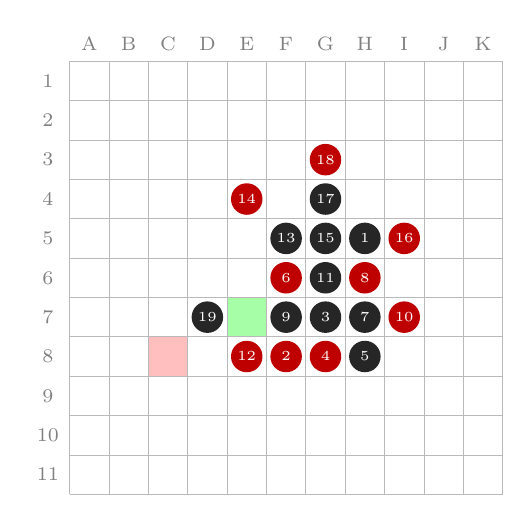
\begin{tikzpicture}[x=.5cm, y=.5cm]
    \fill[red!25] (2,-7) rectangle ++(1,-1);
    \fill[green!35] (4,-6) rectangle ++(1,-1);
    \draw[gray!55, line width=.3pt, step=1] (0,0) grid (11,-11);
    \node[font=\scriptsize, text=gray] at (0.5,.45) {A};
    \node[font=\scriptsize, text=gray] at (-.55,-0.5) {1};
    \node[font=\scriptsize, text=gray] at (1.5,.45) {B};
    \node[font=\scriptsize, text=gray] at (-.55,-1.5) {2};
    \node[font=\scriptsize, text=gray] at (2.5,.45) {C};
    \node[font=\scriptsize, text=gray] at (-.55,-2.5) {3};
    \node[font=\scriptsize, text=gray] at (3.5,.45) {D};
    \node[font=\scriptsize, text=gray] at (-.55,-3.5) {4};
    \node[font=\scriptsize, text=gray] at (4.5,.45) {E};
    \node[font=\scriptsize, text=gray] at (-.55,-4.5) {5};
    \node[font=\scriptsize, text=gray] at (5.5,.45) {F};
    \node[font=\scriptsize, text=gray] at (-.55,-5.5) {6};
    \node[font=\scriptsize, text=gray] at (6.5,.45) {G};
    \node[font=\scriptsize, text=gray] at (-.55,-6.5) {7};
    \node[font=\scriptsize, text=gray] at (7.5,.45) {H};
    \node[font=\scriptsize, text=gray] at (-.55,-7.5) {8};
    \node[font=\scriptsize, text=gray] at (8.5,.45) {I};
    \node[font=\scriptsize, text=gray] at (-.55,-8.5) {9};
    \node[font=\scriptsize, text=gray] at (9.5,.45) {J};
    \node[font=\scriptsize, text=gray] at (-.55,-9.5) {10};
    \node[font=\scriptsize, text=gray] at (10.5,.45) {K};
    \node[font=\scriptsize, text=gray] at (-.55,-10.5) {11};
    \fill[black!85] (7.5,-4.5) circle[radius=.40];
    \node[font=\tiny, text=white] at (7.5,-4.5) {1};
    \fill[red!75!black] (5.5,-7.5) circle[radius=.40];
    \node[font=\tiny, text=white] at (5.5,-7.5) {2};
    \fill[black!85] (6.5,-6.5) circle[radius=.40];
    \node[font=\tiny, text=white] at (6.5,-6.5) {3};
    \fill[red!75!black] (6.5,-7.5) circle[radius=.40];
    \node[font=\tiny, text=white] at (6.5,-7.5) {4};
    \fill[black!85] (7.5,-7.5) circle[radius=.40];
    \node[font=\tiny, text=white] at (7.5,-7.5) {5};
    \fill[red!75!black] (5.5,-5.5) circle[radius=.40];
    \node[font=\tiny, text=white] at (5.5,-5.5) {6};
    \fill[black!85] (7.5,-6.5) circle[radius=.40];
    \node[font=\tiny, text=white] at (7.5,-6.5) {7};
    \fill[red!75!black] (7.5,-5.5) circle[radius=.40];
    \node[font=\tiny, text=white] at (7.5,-5.5) {8};
    \fill[black!85] (5.5,-6.5) circle[radius=.40];
    \node[font=\tiny, text=white] at (5.5,-6.5) {9};
    \fill[red!75!black] (8.5,-6.5) circle[radius=.40];
    \node[font=\tiny, text=white] at (8.5,-6.5) {10};
    \fill[black!85] (6.5,-5.5) circle[radius=.40];
    \node[font=\tiny, text=white] at (6.5,-5.5) {11};
    \fill[red!75!black] (4.5,-7.5) circle[radius=.40];
    \node[font=\tiny, text=white] at (4.5,-7.5) {12};
    \fill[black!85] (5.5,-4.5) circle[radius=.40];
    \node[font=\tiny, text=white] at (5.5,-4.5) {13};
    \fill[red!75!black] (4.5,-3.5) circle[radius=.40];
    \node[font=\tiny, text=white] at (4.5,-3.5) {14};
    \fill[black!85] (6.5,-4.5) circle[radius=.40];
    \node[font=\tiny, text=white] at (6.5,-4.5) {15};
    \fill[red!75!black] (8.5,-4.5) circle[radius=.40];
    \node[font=\tiny, text=white] at (8.5,-4.5) {16};
    \fill[black!85] (6.5,-3.5) circle[radius=.40];
    \node[font=\tiny, text=white] at (6.5,-3.5) {17};
    \fill[red!75!black] (6.5,-2.5) circle[radius=.40];
    \node[font=\tiny, text=white] at (6.5,-2.5) {18};
    \fill[black!85] (3.5,-6.5) circle[radius=.40];
    \node[font=\tiny, text=white] at (3.5,-6.5) {19};
  \end{tikzpicture}
  \caption{Ván 26, thế trước nước 20. L8 (O, quân đỏ) đi C8 (ô đỏ nhạt) trong khi E7 (ô xanh) là ô thắng ngay duy nhất của AlphaBeta (X, quân đen).}
  \label{fig:van26}
\end{figure}
